\documentclass{article}[twocolumn]
\usepackage[pdftex]{graphicx}
\usepackage[utf8]{inputenc}
\usepackage[brazil]{babel}
\usepackage{subfigure}
\usepackage{mathtools}
\usepackage{amsmath}
\usepackage{amssymb}
\usepackage{float}
\usepackage{tikz}

\title{Cores do VSS}
\author{Kenji Yamane}

\definecolor{vssgreen}{RGB}{0, 255, 0}
\definecolor{vsspurple}{RGB}{168, 122, 255}
\definecolor{vssorange}{RGB}{255, 128, 0}
\definecolor{vsspink}{RGB}{255, 51, 255}
\definecolor{vssblue}{RGB}{0, 0, 255}
\definecolor{vssyellow}{RGB}{255, 255, 51}
\definecolor{vsscyan}{RGB}{145, 255, 245}
\definecolor{vssred}{RGB}{255, 0, 0}
    
\begin{document}
	Possibilitando de forma efetiva a utiliza\c{c}\~ao da c\^amera pessoal do
	computador, estudando os espa\c{c}os de cores RGB, YUV e HSV, e criando
	devidamente as fun\c{c}\~oes de convers\~ao entre os espa\c{c}os de cores
	HSV e YUV, p\^ode-se efetivar a convers\~ao do calibrador de cores do VSS
	para HSV. Inicialmente ele estava funcionando tendo como base somente o espa\c{c}o
	YUV. A figura \ref{fig:cali_yuv} mostra o calibrador neste estado original.
	\begin{figure}[H]
		\centering
		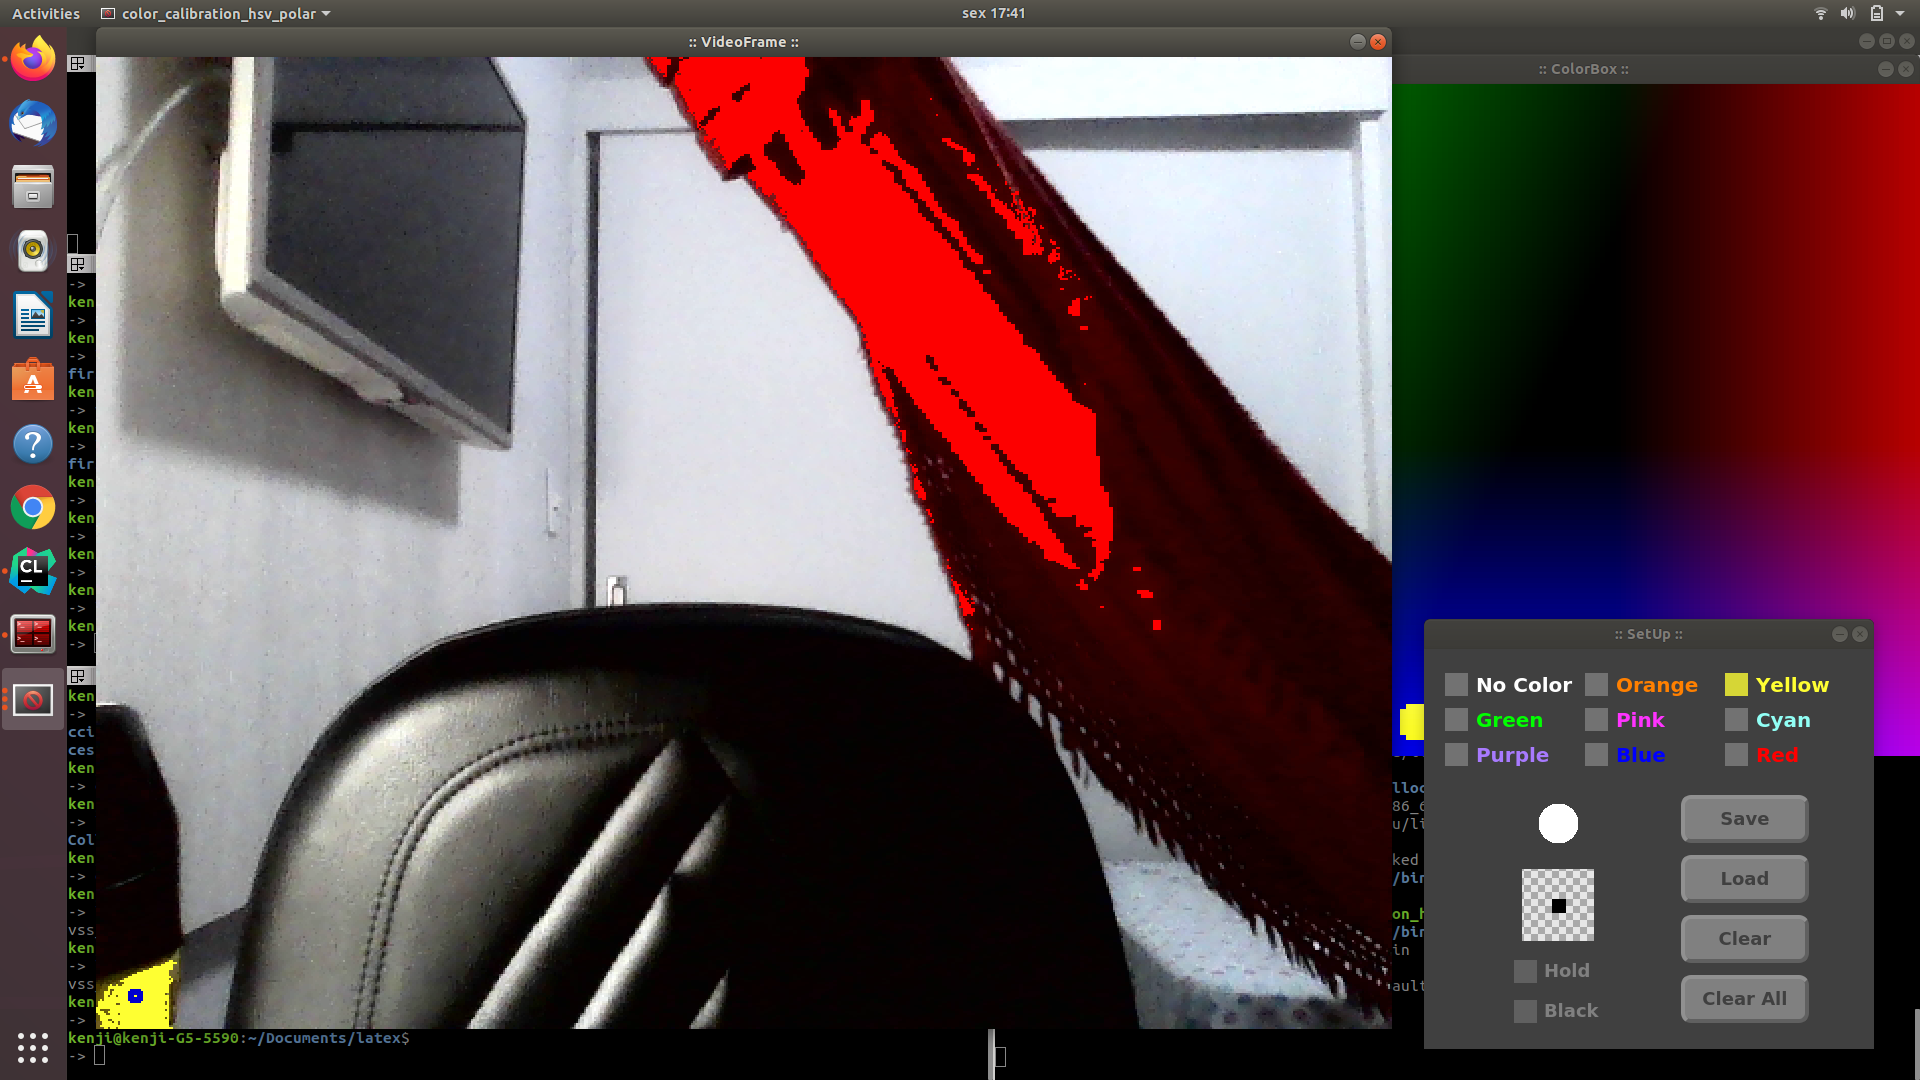
\includegraphics[width=10cm]{color_calibrator_yuv.png}
		\caption{Calibrador de cores do VSS em YUV}
		\label{fig:cali_yuv}
	\end{figure}
	A tela maior corresponde \`a vis\~ao da c\^amera, onde se pode classificar os canais y, u e v
	de determinados pixels dela como uma das 8 cores que est\~ao mostradas na tela menor, basta
	clicar nos pixels que se quer classificar (na figura, pode-se ver parte dos pixels
	classificados como vermelho e parte classificados como amarelo). A tela menor funciona para
	escolher a cor para a qual ser\~ao segmentados os pixels clicados na tela maior, assim como
	salvar ou carregar ou limpar segmenta\c{c}\~oes pr\'evias. A tela de tamanho intermedi\'ario
	mostra um corte vertical do cubo YUV, com o canal y no eixo vertical. Pode-se alterar a
	se\c{c}\~ao y mostrada com o \textit{scroll} do \textit{mouse}. A caixa YUV em mais detalhes
	\'e mostrada na figura \ref{fig:box_yuv}.
	\begin{figure}[H]
		\centering
		\subfigure[y m\'inimo]{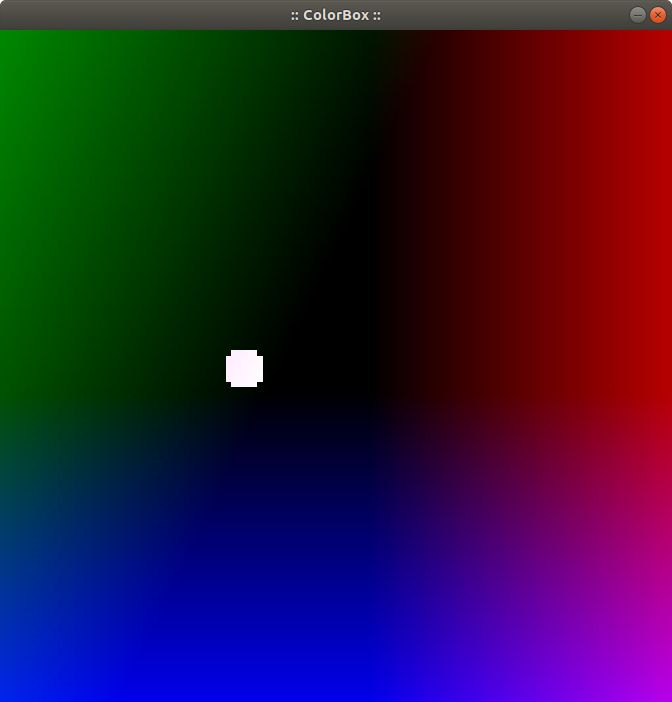
\includegraphics[width=3cm]{yuvbox_low.png}}
		\subfigure[y intermedi\'ario]{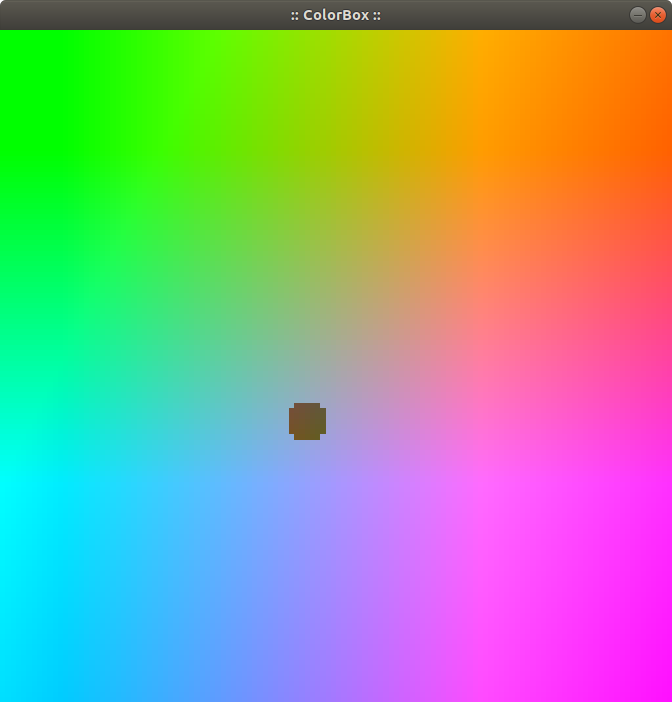
\includegraphics[width=3cm]{yuvbox_mid.png}}
		\subfigure[y m\'aximo]{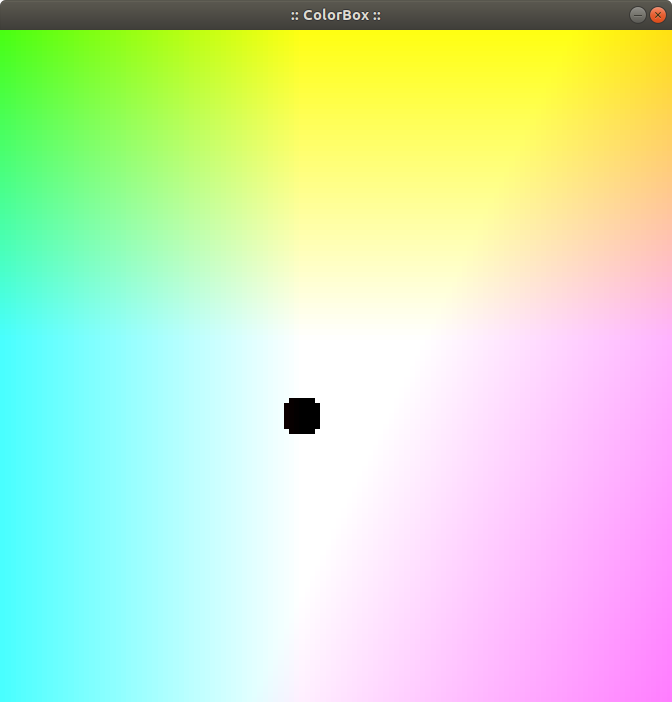
\includegraphics[width=3cm]{yuvbox_big.png}}
		\caption{Curvas de n\'ivel da caixa YUV}
		\label{fig:box_yuv}
	\end{figure}
	Agora para a vers\~ao HSV, decidiu-se ao inv\'es de converter totalmente a ferramenta
	de calibra\c{c}\~ao para HSV, refatorar o c\'odigo para suportar os dois modos: YUV e HSV.
	Para este fim, utilizou-se algumas vezes uma vari\'avel de um \textit{singleton} para poder
	realizar condicionais que ramificam o c\'odigo ou para YUV ou para HSV e tamb\'em
	transformou-se algumas classes da ferramenta em uma abstrata e duas derivadas, uma para YUV
	e uma HSV. O seguinte padr\~ao de cores foi imprimido para poder se verificar melhor a
	efic\'acia da ferramenta para segmentar as cores, permitindo verificar se algum erro foi
	cometido.
	\begin{center}
		\begin{tikzpicture}[scale=0.20]
			\filldraw [vssgreen] (0, 0) circle (2);
			\filldraw [vsspurple] (7, 0) circle (2);
			\filldraw [vssorange] (0, 5) circle (2);
			\filldraw [vsspink] (7, 5) circle (2);
			\filldraw [vssblue] (0, 10) circle (2);
			\filldraw [vssyellow] (7, 10) circle (2);
			\filldraw [vsscyan] (0, 15) circle (2);
			\filldraw [vssred] (7, 15) circle (2);
		\end{tikzpicture}
	\end{center}
	Por\'em, ao buscar se utilizar o HSV no seu espa\c{c}o nativo, um cilindro, observou-se
	que a ferramenta tinha dificuldade em atribuir cores para algumas triplas (h, s e v). Esse
	problema se manifesta tamb\'em na representa\c{c}\~ao do cilindro HSV, mostrado na figura
	\ref{fig:hsv_buggy}.
	\begin{figure}[H]
		\centering
		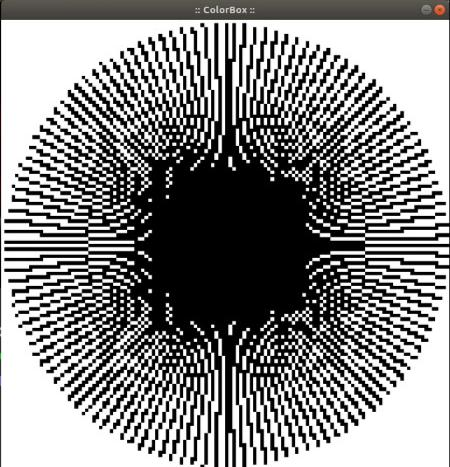
\includegraphics[width=3cm]{hsvcyl_low_buggy.png}
		\caption{Cilindro HSV com falhas}
		\label{fig:hsv_buggy}
	\end{figure}
	Onde se pode concluir que isso s\~ao consequ\^encias do \^angulo (\textit{hue}) ser discretizado
	de forma igual ao raio (\textit{saturation}). Pode-se mitigar este efeito aumentando os bits
	reservados para apresentarem cada canal (no momento 7 bits para cada um). Por\'em isso teria
	repercuss\~oes em c\'odigos compartilhados por todas as categorias da iniciativa, sendo que
	algumas n\~ao poderiam lidar com um uso de mem\'oria mais alta. Sendo assim, decidiu-se ao
	inv\'es disso trabalhar com o espa\c{c}o HSV diretamente com os valores (h, s, v) representados
	em um cubo, de forma parecida ao YUV. O resultado \'e mostrado na figura \ref{fig:cyl_hsv}.
	\begin{figure}[H]
		\centering
		\subfigure[v m\'inimo]{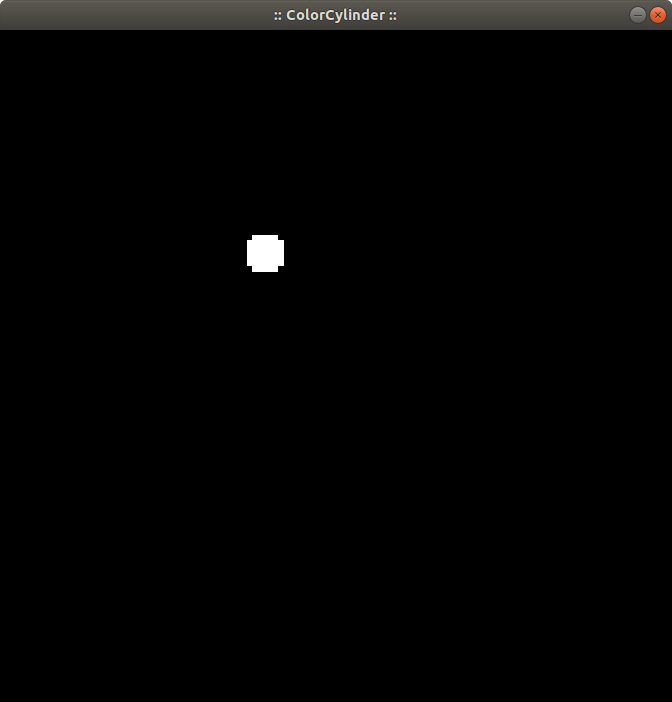
\includegraphics[width=3cm]{hsvcyl_low.png}}
		\subfigure[v intermedi\'ario]{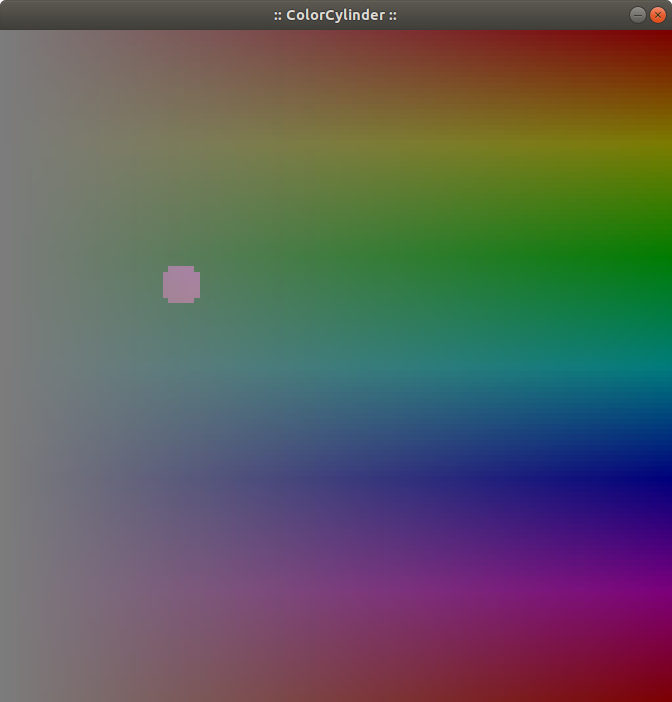
\includegraphics[width=3cm]{hsvcyl_mid.png}}
		\subfigure[v m\'aximo]{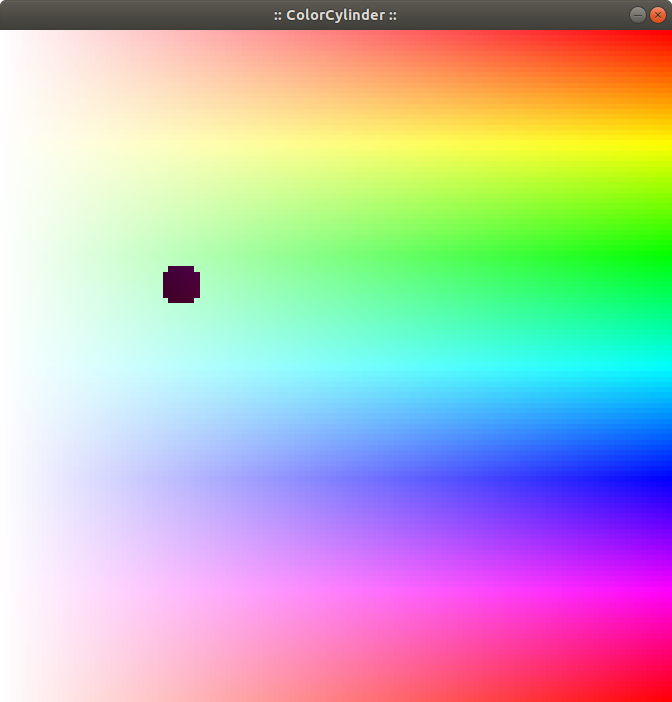
\includegraphics[width=3cm]{hsvcyl_big.png}}
		\caption{Curvas de n\'ivel do cilindro HSV}
		\label{fig:cyl_hsv}
	\end{figure}
	Apesar dele aparentar n\~ao ser euclidiano, em compara\c{c}\~ao com o cilindro, e apresentar
	um vi\'es para o branco, observa-se que os problemas encontrados com o cilindro deixam
	de existir.

	Trabalhando-se desta forma pode-se verificar como o espa\c{c}o HSV \'e certamente bem mais
	organizado com rela\c{c}\~ao as cores, assim como sua rela\c{c}\~ao com a ilumina\c{c}\~ao
	(o canal \textit{value}), mostrando-se mais prop\'icio para algoritmos de compensa\c{c}\~ao
	de ilumina\c{c}\~ao. Como esta ver\~ao linearizada do HSV n\~ao gerou os mesmos \textit{bugs}
	que o cilindro, utilizar-se-\'a esta vers\~ao. Desta forma, adicionou-se efetivamente o
	modo HSV \`a ferramenta de calibra\c{c}\~ao do VSS. Pretendo, no m\^es de fevereiro, j\'a
	iniciar os estudos de poss\'iveis algoritmos de compensa\c{c}\~ao de ilumina\c{c}\~ao e
	realizar tentativas de implement\'a-los e integr\'a-los \`a ferramenta.
\end{document}
